\chapter{Pràctica}
\section{Placa base CC1352R1}
Per analitzar el protocol BLE i veure les seves característiques s'ha utilitzat el kit per desenvolupament ràpid del microcontrolador CC1352R1.
\begin{figure}[h!]
	\begin{center}
		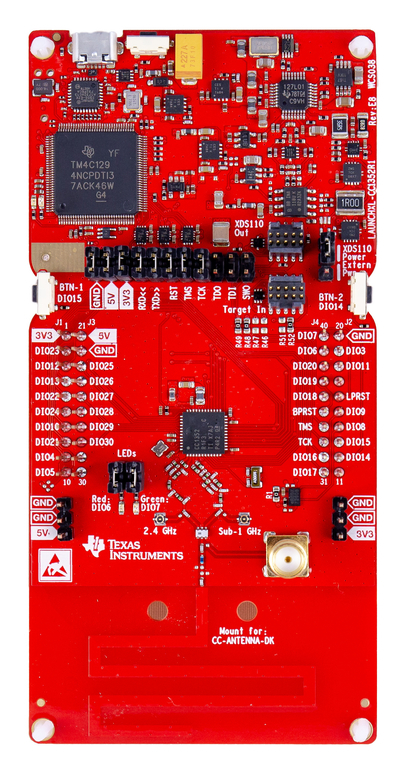
\includegraphics[width=0.5\textwidth]{./images/launchxl-cc1352r1.jpg}
		\caption{Placa \cite{placa}}
	\end{center}
\end{figure}

Aquesta placa permet el desenvolupament d'aplicacions en BLE utilitzant el microcontrolador CC1352 de Texas Instruments a continuació es descriuen les seves característiques principals \cite{placa_datasheet}.

El dispositiu CC1352R és multiprotocol i multibanda orientat a 2.4 GHz o sub-1GHz que serveix per a Thread, Zigbee, Bluetooth 5 Low Energy, IEEE 802.15.4g i 6LoWPAN. Pel que fa a memòria té 352 KB flash programable, 256 KB de ROM per a protocols i llibreries, 8 KB de Cache SRAM i 80 KB de RAM protegida amb paritat.
Pel que fa als perifèrics el més important és el ADC de 12 bits i 8 canals amb freqüència de mostreig de 200 Kmostres/s (multiplexat). També té Rellotge de Temps Real (RTC), acceleradors de operacions criptogràfiques i generador de números aleatoris.
La radio multibanda que té te un receptor amb sensibilitat de -121 dBm per a sub-1GHz i de -110 dBm a 50 Kbps o -105 dBm a 125 Kbps. El transmissor pot transmetre fins a 14 dBm sub-1GHz i 5dBm a 2.4 GHz.


\section{Software}
Per al desenvolupament de projectes per a la placa s'ha utilitzat el entorn de desenvolupament Code Composer Studio. El software és el SimpleLink(TM) CC13X2.
[Comentar tema versió]

\section{Project 0}
El Project 0 és el projecte instal·lat amb que les plaques vénen de fàbrica. Aquest projecte exposa certs serveis a través de BLE i et permet veure una comunicació simple entre la placa i un dispositiu mòbil.
La comunicació es fa a través del control dels dos LEDs que te la placa (els LEDs que estan directament controlats pel microcontrolador) i també per l'estat dels botons que hi ha a ambdós costats de la placa.
*Aquest projecte també inclou altres serveis en que no entrarem.

Aquest projecte serveix per tenir un bon exemple de com està dissenyada l'arquitectura dels serveis amb les seves característiques amb una relativa simple funcionalitat. A continuació s'analitzaran diferents parts dels atributs.

\subsection{Serveis de Butons i LEDs}

En la següent taula es poden veure tots els valors que hi ha tal i com estan en la taula d'atributs del servidor GATT.
Per facilitar la visualització de les dades s'han tret els zeros finals dels UUIDs propis però cal recordar que en total tenen 16 parells (128 bits en representació hexadecimal) i no només els 9 parells que surten a la taula.

\begin{center}
	\begin{table}[h!]
		\csvautotabular{data_files/projectzeroUUID.csv}
	\end{table}
\end{center}

Per poder entendre els atributs, al tenir UUID propis és necessari tenir en compte la documentació amb la que s'ha desenvolupat aquest projecte.

\begin{figure}[h!]
	\begin{center}
		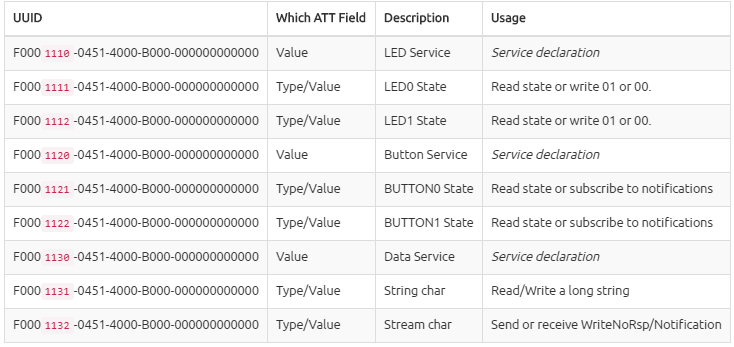
\includegraphics[width=\textwidth]{./images/Project_0_UUID.png}
		\caption{Definició dels UUIDs}
	\end{center}
\end{figure}

El primer que cal tenir clar és que en taula anterior (afegir link dinàmic) els valors estan representats amb l'ordre en que es reben i en general els serveis estandarditzats (i també aquest servei propi) utilitza \textit{little-endian} per enviar la informació.
Això resulta en que els caràcters hexadecimals queden (per parelles) ordenats al revés.

Al analitzar els atributs es pot veure com aquells que tenen el UUID 0x2800 en el seu valor només tenen un UUID corresponent al les definicions de serveis de LEDs i de botons.
Seguidament, als atribut amb UUID 0x2803 hi ha les definicions de les característiques, en el seu valor hi ha múltiples parts.
El primer parell hexadecimal correspon a les propietats. Just després hi ha dos parells hexadecimals que identifiquen el \textit{Handle} del atribut on hi ha la característica.
I per últim la resta de caràcters corresponen al UUID que identifica la característica.

\subsection{Propietats}
Les propietats d'accés són un valor que identifica quines operacions i procediments es poden fer sobre la característica.
El camp té 8 bits per defecte i cada un d'ells identifica una operació o procediment.
Es poden combinar qualsevol quantitat d'aquests bits per habilitar múltiples opcions.

\begin{center}
	\begin{tabular}{|c|c|l|}
		\hline
		Binary	&	Hex		&	Property	\\	\hline
		0000 0001	&	0x01	&	Broadcast\\	\hline
		0000 0010	&	0x02	&	Read	\\	\hline
		0000 0100	&	0x04	&	Write w/o Response	\\	\hline
		0000 1000	&	0x08	&	Write	\\	\hline
		0001 0000	&	0x10	&	Notification w/o ACK	\\	\hline
		0010 0000	&	0x20	&	Indication with ACK	\\	\hline
		0100 0000	&	0x40	&	Signed Writes	\\	\hline
		1000 0000	&	0x80	&	Aditional Properties	\\	\hline
	\end{tabular}
\end{center}

Primer de tot cal destacar la implementació de comunicacions amb o sense reconeixement. D'aquesta manera si preferim reduir la quantitat de missatges per estalviar bateria enlloc d'assegurar-se que s'ha rebut la informació es dona la opció.

Pel que fa les propietats en el Project 0 les característiques dels LEDs tenen el valor 0x0E que resulta en 0000 1110 per tant, es permet: llegir, escriure i escriure sense resposta.
En canvi les característiques del servei de botons té el valor 0x12 que suposa 0001 0010, per tant, es permet notificació sense reconeixement.

La notificació i indicació són funcions que ajuden a reduir el consum de recursos.
Quan volem saber en quin estat estan els botons de la placa contínuament es podria anar llegint el estat de la característica constantment però això suposarien molts missatges i reduiria el temps que els dispositius es poden adormir i així ser més eficients.
Per evitar aquest cas es pot configurar la característica tal que sigui la mateixa placa qui enviï el missatge automàticament quant el estat de la característica canviï.
D'aquesta manera el receptor només cal que escolti els missatges de la placa per tal de saber en quin estat està el botó.

En cas de que es vulgui indicació amb reconeixements és possible configurar-ho d'aquesta manera a través del atribut Configuració de Característica del Client identificat amb el UUID 0x2902 i estandarditzat en la especificació de Bluetooth.
Si el valor és 0 no hi ha transmissions, si el valor és 1 s'envien notificacions (sense reconeixement) i si el valor és 2 s'envien indicacions (notificacions amb reconeixement). 

El bit d'extensió de propietats, en cas que sigui 1 indica que existeix un atribut: Descriptor Propietats Esteses de Característica.
Aquest atribut te el UUID 0x2900 i el que permet és afegir més propietats de les que poden existir amb el espai limitat de 8 bits que hi ha per defecte.
Aquest sistema permet afegir fins a 16 bits més per indicar propietats, ara per ara estan els dos primers definits segons el estàndard i la resta estan reservats per a ús futur \cite{extended properties}.

